\documentclass{article}

\usepackage{amsmath}
\usepackage{parskip}
\usepackage{siunitx}
\usepackage{subcaption}
%\usepackage{beramono}
\usepackage{graphicx}
\usepackage{listings}
\usepackage[usenames,dvipsnames]{xcolor}

\newcommand{\del}[2]{\frac{\partial #1}{\partial #2}}  % Partial derivative
\newcommand{\deriv}[2]{\frac{\mathrm{d} #1}{\mathrm{d} #2}}  % Derivative
\newcommand{\dderiv}[2]{\frac{\mathrm{d}^2 #1}{\mathrm{d} #2^2}}  % Second derivative
\newcommand{\expval}[1]{\langle #1 \rangle}

%%
%% Julia definition (c) 2014 Jubobs
%%
\lstdefinelanguage{Julia}%
  {morekeywords={abstract,break,case,catch,const,continue,do,else,elseif,%
      end,export,false,for,function,immutable,import,importall,if,in,%
      macro,module,otherwise,quote,return,switch,true,try,type,typealias,%
      using,while},%
   sensitive=true,%
   alsoother={$},%
   morecomment=[l]\#,%
   morecomment=[n]{\#=}{=\#},%
   morestring=[s]{"}{"},%
   morestring=[m]{'}{'},%
}[keywords,comments,strings]%

\lstset{%
    language         = Julia,
    basicstyle       = \ttfamily,
    keywordstyle     = \bfseries\color{blue},
    stringstyle      = \color{magenta},
    commentstyle     = \color{ForestGreen},
    showstringspaces = false,
}
\title{Exam Computational Physics\\
  2020}
\author{Thorvald M. Ballestad}

\begin{document}
\maketitle
\begin{abstract}
  Metropolis Monte Carlo simulation of 2D Ising model, using the Mon-Jasnow and extended Mon-Jasnow algorithm.
  This report is not intended as a scientific report, but as an answer to the exam.
  The goal of this report is to give a brief overview of how I have solved the problem, and then go into the parts of the solution that I think are the most interesting.
  Thus, this report consists of a brief documentation of the code and then explanations and thought on the interesting aspects of the solution.
\end{abstract}

\section{Overview of the code}
The simulation is written in Julia and the plots are generated in Python.
As the Python code is just simple plotting, I will not give it much focus here.
The code is separated into files, the main part being in \verb|utils.jl|.
Nothing should be run directly from \verb|utils.jl|, it contains the machinery that can be used from other designated scripts.
For each type of ``operation'' that we want to execute, there should exist a file, that extends \verb|utils.jl|, for example \verb|task1.jl| and \verb|investigate_error.jl|.

Firstly, a \emph{very} brief explanation of the Metropolis method.
Given a 2D Ising lattice, select at random one lattice site.
For this site, determine the change of energy in the system if one were to flip this spin.
If the change in energy is negative, accept the flip.
If it is positive, let the probability of flipping it be given by the Boltzmann distribution.
A natural definition of a time step is a sweep, defined as $N^2$ flip attempts, where $N$ is the dimension of the lattice.
In the Mon-Jasnow and extended Mon-Jasnow algorithm, one applies the Metropolis method to certain lattice, that is such that there exists another lattice of close resembelance, but for which there exists an interface.
It can be shown that the tension $\tau$ is a function of the difference in energy of the two systems.

There are a number of tricks one might use to improve performance.
Some of these come from insigth to the problem itself and some are of more programatic nature.
As examples of tricks from insight into the problem are generating a table of possible $e^{\Delta H/T}$ values, that are used in the flip attempt, and how one calculates the energy difference.
As a flip will only affect the nearest neighbors (the definition of Ising model), there are only a few possible values for the Boltzmann weights.
In fact, as we allways accept flips with negative energy change, the only values that needs calculating are $e^{-8/T}$ and $e^{-4/T}$.
As expontents are computational heavy, this gives a big performance boost.


As for the energy calculation one has several options.
The naive implementation would calculate the energy of the entire spin matrix for each measurement.
However, a better approach is to measure only the inital energy, and then cumulatively add the energy change from each flip.
In our problem, the energy is not really needed, except for debugging and determining when the system reaches equilibrium.
The only quantity of importance, is the difference in energy between the two systems that the Mon-Jasnow algorithm considers -- fixes positive and negative sides for original Mon-Jasnow, and torus and klein flask for the extended algorithm.
These energy differences have simple formulas: two time the magnetization of the rightmost column for the original, as stated in \cite{mon_jasnow}, and for the extended I found the expression
\begin{equation}
  \sum_y S_{1,y} [ S_{N_x, y} + S_{N_x, N_y+1-y} ],
\end{equation}
which is stated without proof.
As Julia is column oriented in its arrays, this ends up being very efficient to calculate.

Now to the more programatic aspects of my solution.
There are some solutions in particular that I would like to emphasise.
Here I will not discuss the performance in detail, for that see \ref{sec:performance}.
Firstly, the code is written in a very modul based manner.
This makes it easy to change, both cosmetic changes to code and alterations to how one calculates or represents data.
This gives a very general code, for which I am proud.
When going from the original algorithm to the extended, only the input data must be changed, the code stays the same.
This was also very helpful when performing benchmarks and improving performance.

One of the programatic challanges in this problem is the boundary conditions.
When calculating neighbor interaction one has to know what the neighbors are.
Most implementations would problably, even though there are other possibilities, store the spin information in a two dimensional array, maintaining position information from the system in the data structure.
A first naive approach to the boundary conditions would be to for each flip attempt check if one is at a boundary.
Firstly, this could give more complicated code, and also it would have to be rewritten for each type of system.
Secondly, it would involve checking several conditions, and if one is at the border, additions.
In my solution, inspired by excercise 1 in this curse, the position information of the data structure is disregarded, at least when checking neighbor interaction.
For each direction, right, left, up, down, there is a vector that gives the next index.
For example, if you are at position $(x, y)$, the next position to the right would be $(\text{ir}(x), y)$, where \verb|ir| is the vector that gives the index to the right.
Normally, \verb|ir| at index $i$ is simply $i+1$, likewise for down, \verb|id| at index $j$ is $j-1$.
However, at the boundaries, the index is such that the boundary condition is met, for example the right index at the rightmost postion $N_x$ would be 1.
A point of note is that the left and right position is only dependent on $x$ and likewise up and down is only dependent on $y$.
Thus, the sites can be connected in whatever order one wishes, but only in $x$ and $y$ independently -- the data are like two graphs, one for $x$ and one for $y$.
At one point, I had the structure so that it was only one graph, the right position was dependent on both $x$ and $y$, and would give new values for $x$ and $y$, allowing arbitrary geometries.
This would be necessary for the klein bottle geometry, for example, where going right may change the position in $y$.
However, since one never has to do any calculations on the klein system, only the torus, I chose to reduce the generality of my solution in favor of performance.
These vectors, describing the structure of the graph, will from here on be refered to as index vectors.

The index vectors are central in my solution to setting up the fixed positive and negative columns of the original Mon-Jasnow algorithm.
When selecting a lattice point at which to attempt a flip, I generate a random number between one and the number of lattice points in my system.
In the original Mon-Jasnow the site to flip cannot, of course, be one of the fixed columns.
In the interest of keeping the code general, my solution is somewhat less intuitive, but still highly efficient.
Since we choose a random number between 1 and $N^2$, the first $N^2$ numbers must be non-fixed, and the fixed columns must be placed at the end of the array.
As Julia is column based, this corresponds to columns after the Nth column.
One could of course ommit this by generating a number between a given number and some other given number, but in my opinion, that would be less clean code.
The solution is to add a positive column at the end, ie. to the right, of the spin array.
We do not need a negative column, as one never simulates on the positive/negative system, only the positive/positive.
Using the index vectors, this column is placed \emph{both} to the right and to the left of the system.
The index right vector at position $N_x$ gives $N_{x+1}$ where the positive column is.
The clever part is that the index left vector at position $1$ is $N_{x+1}$!
Finally, to make this solution work completely, energy calculation has to be considered.
Given a spin configuration array, it is simple to calculate the total energy -- simply sum over all neighbor interactions.
To maintain general code, this sum would also run over the fixed column on the right (remember, I now talk about the position in actual memory, so the left column does not exist here. But for neighbor interaction in the calculation, the index vectors are used).
The right column has no neighbor on the right, it is not a part of the system!
Here, the solution is again the index vectors, because the index vector right at positon $N_{x+1}$ is $N_{x+1}$!
This simply lead to a constant addition in the energy, which we of course are allowed to do.


Measurements are not always trivial for Monte Carlo simulations.
There are mainly two aspects of interest, the equilibration time and correlation time.
When startig the simulatoin, it must be run for some period of time before the system has reached equilibrium.
Before this point, it makes no sense to take samples for calculating expectation value.
Also, after a measurement, one should wait some period of time before making a new measurement, to ensure that the two states are not correlated.
One might do alot of work on these aspects.
For example, for finding equilibrium time, one solution is to simulate two different initial conditions, and see when the energy of the two systems stamilize at the same level.
I did this in order to find an approximate value, but another solution, which would require some more computation time, would be to do this every time one ran the system, and use the collected data to infer when to begin measurements.
Also, much more work could be done in finding a correlation time.
I did this quite naively, simply measuring every three sweeps.
\cite{niels} had quite a bit of discussion on this point, and concluded that it would often be sufficient to sample every sweep for Metropolis.
It is possible that one could get better results if one had put more work into this, but I believe it would take quite alot more time and also would require spending more time understanding the physics fully.

For obtaining error estimates, I used the Bootstrap methdo, described in \cite{niels}.
It is not perfect, for example it is heavily dependent on the number of resaples, I do 700, but it does at the very least give an indication of relative uncertainty between simulations.
The method is quite computational demanding, for low values of the lattice size $N$ the Bootstrapping take more time than the simulation.


- Bootstrap and measurements

Interesting solutions:
- Indexes for neighbor points
- Very modul based code.
  |-> Was very easy to implement new types of index vectors
- Does not really need energy, only the energy difference, which can be calulated explicitly every sweep
- Exponent lookup
- delta_H_sweep allocated outside loop
- Solution to ++ +- boundaries


\section{Results}


\begin{figure}[ht]
  \centering
  \subcaptionbox{Torus}{
    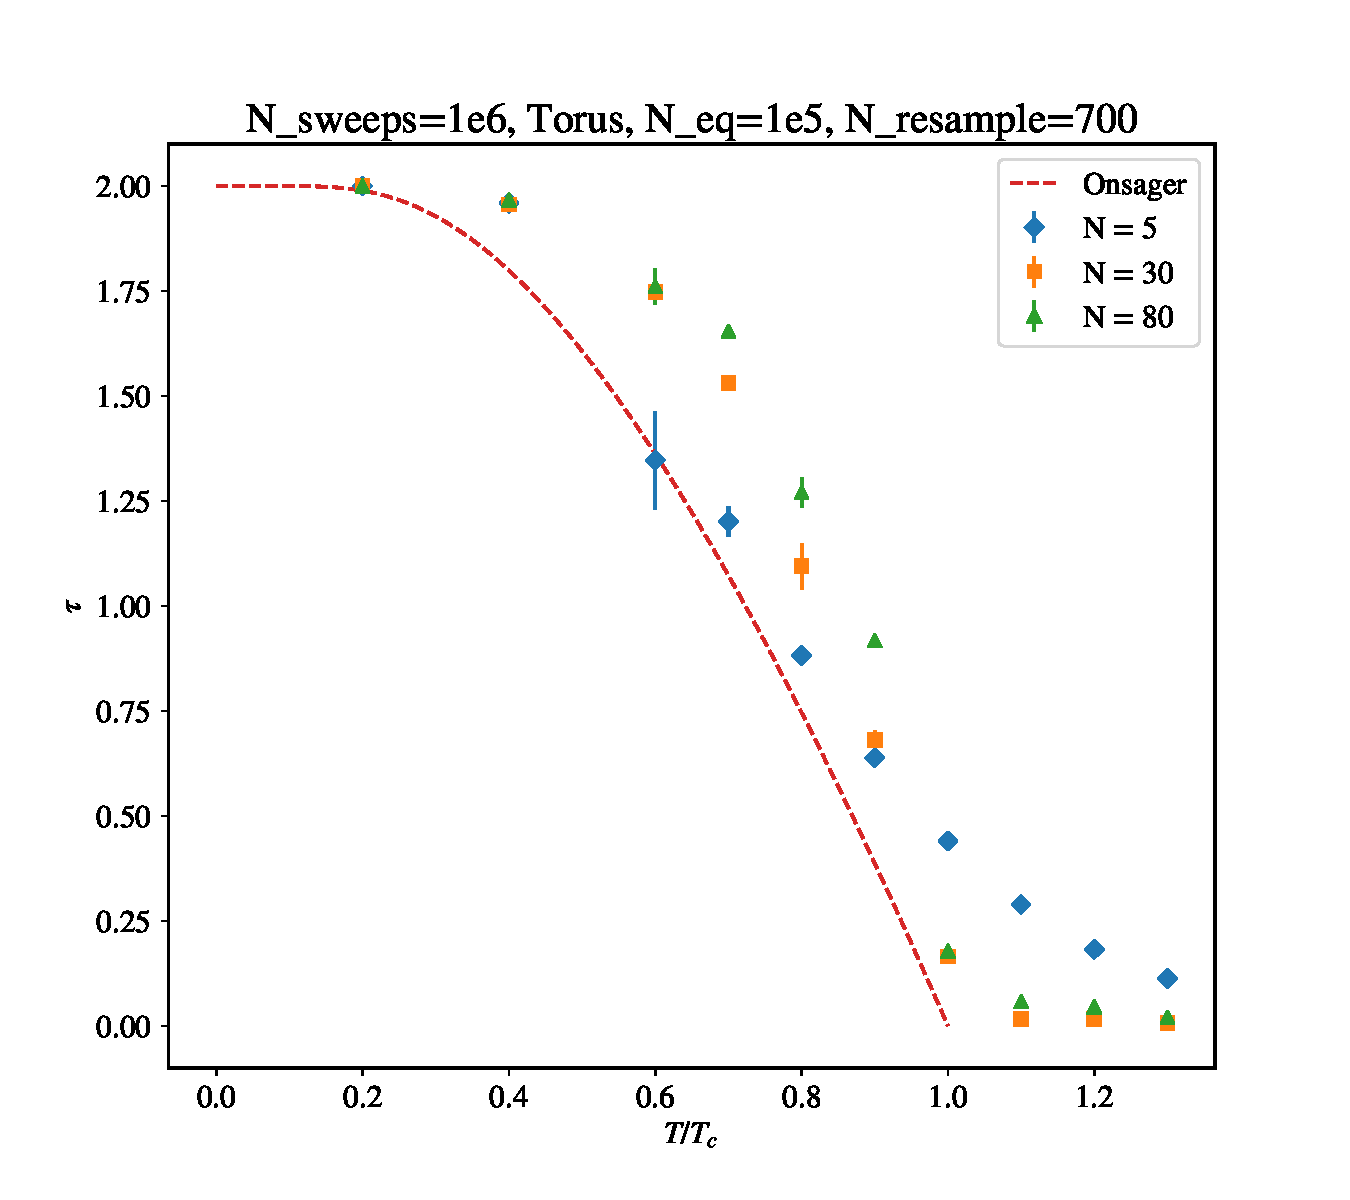
\includegraphics[width=.47\textwidth]{media/tau_T_torus}
  }
  \subcaptionbox{PP}{
    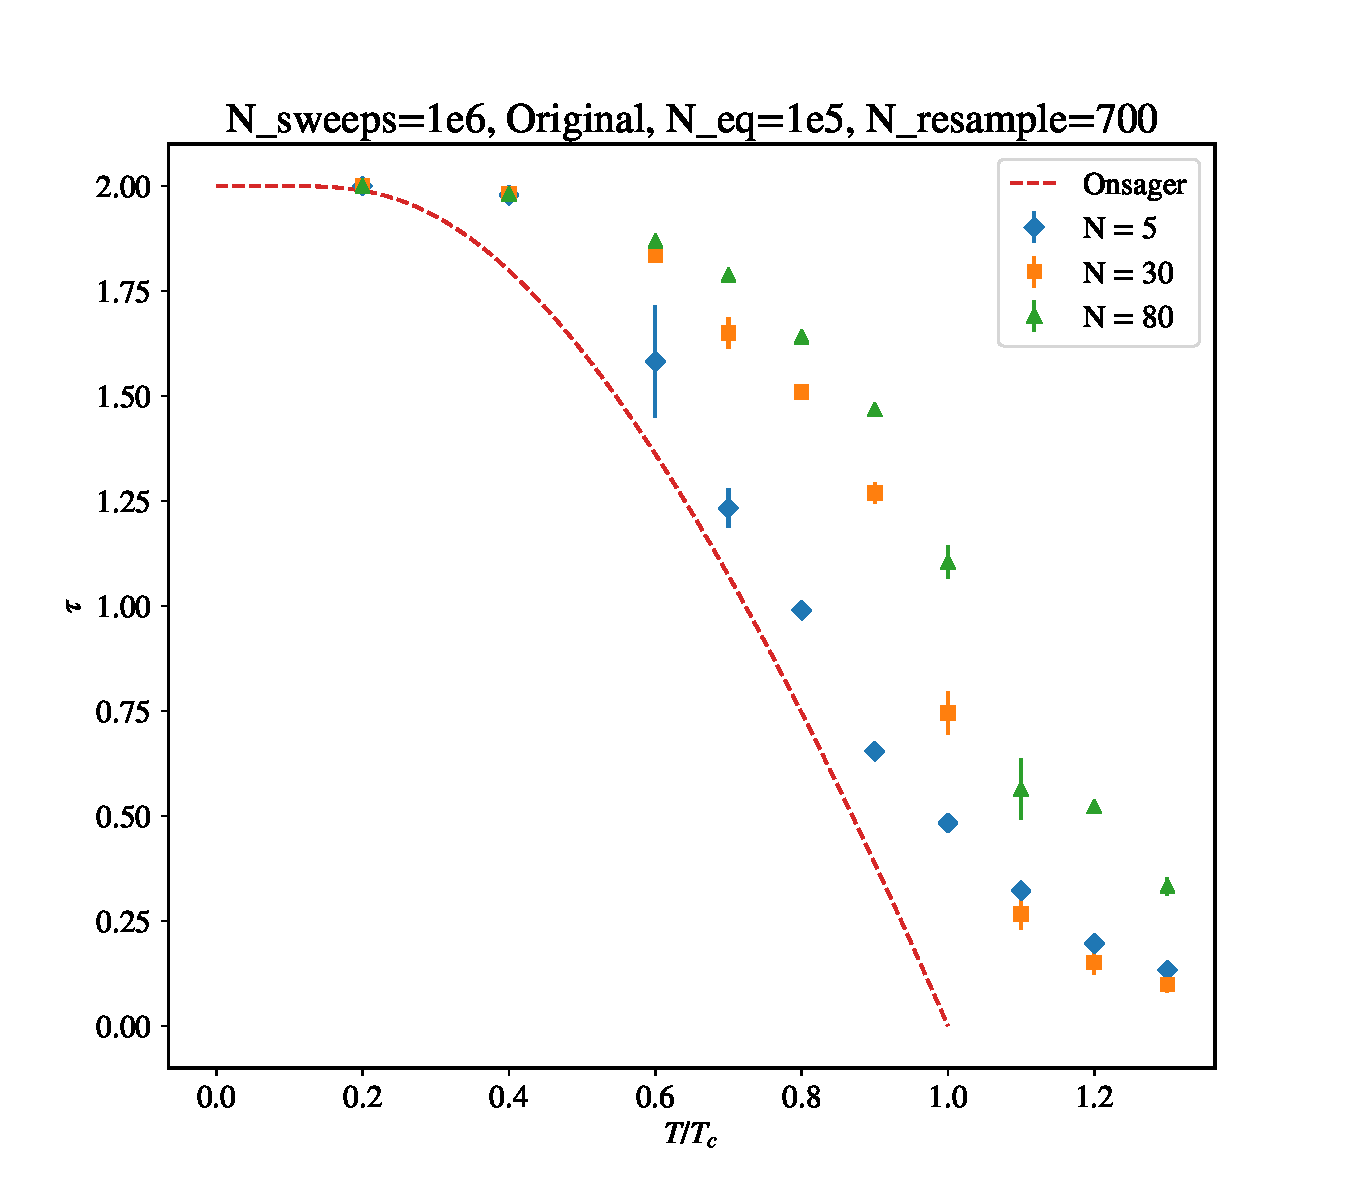
\includegraphics[width=.47\textwidth]{media/tau_T_pp}
  }
  \caption{$\tau$ as a function of T.\label{fig:tau_T}}
\end{figure}

\begin{figure}[ht]
  \centering
  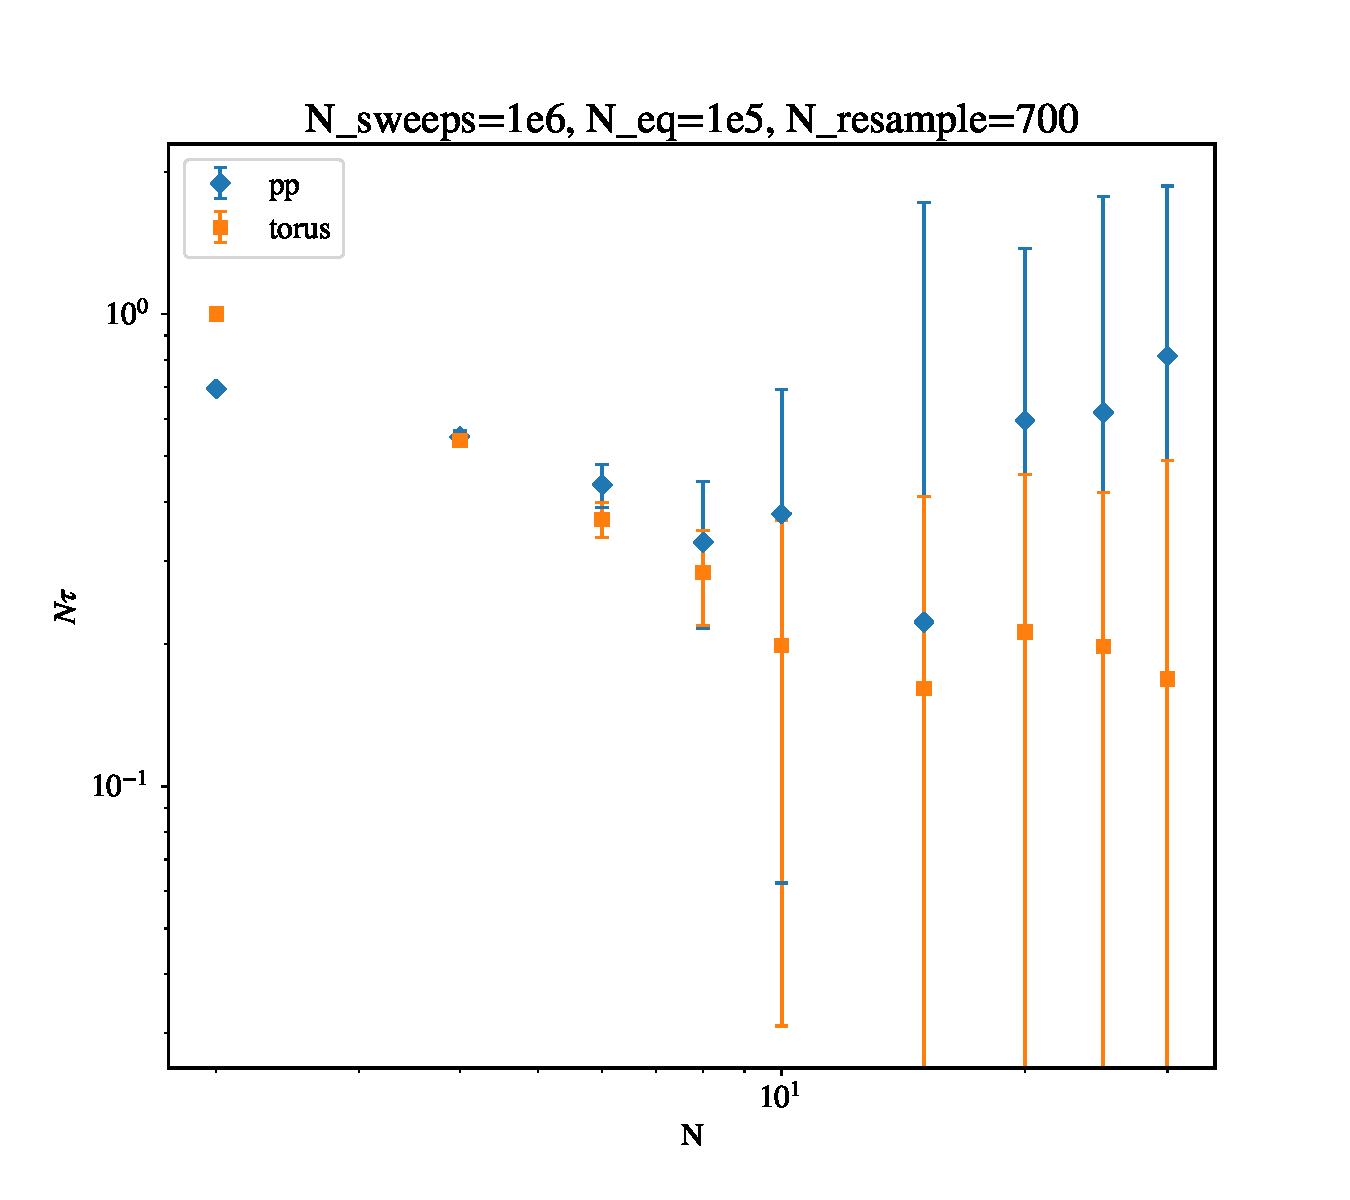
\includegraphics[width=.75\textwidth]{media/tau_N}
  \caption{$N\tau$ as a function of N for $T=T_c$.\label{fig:tau_N}}
\end{figure}

\begin{figure}[ht]
  \centering
  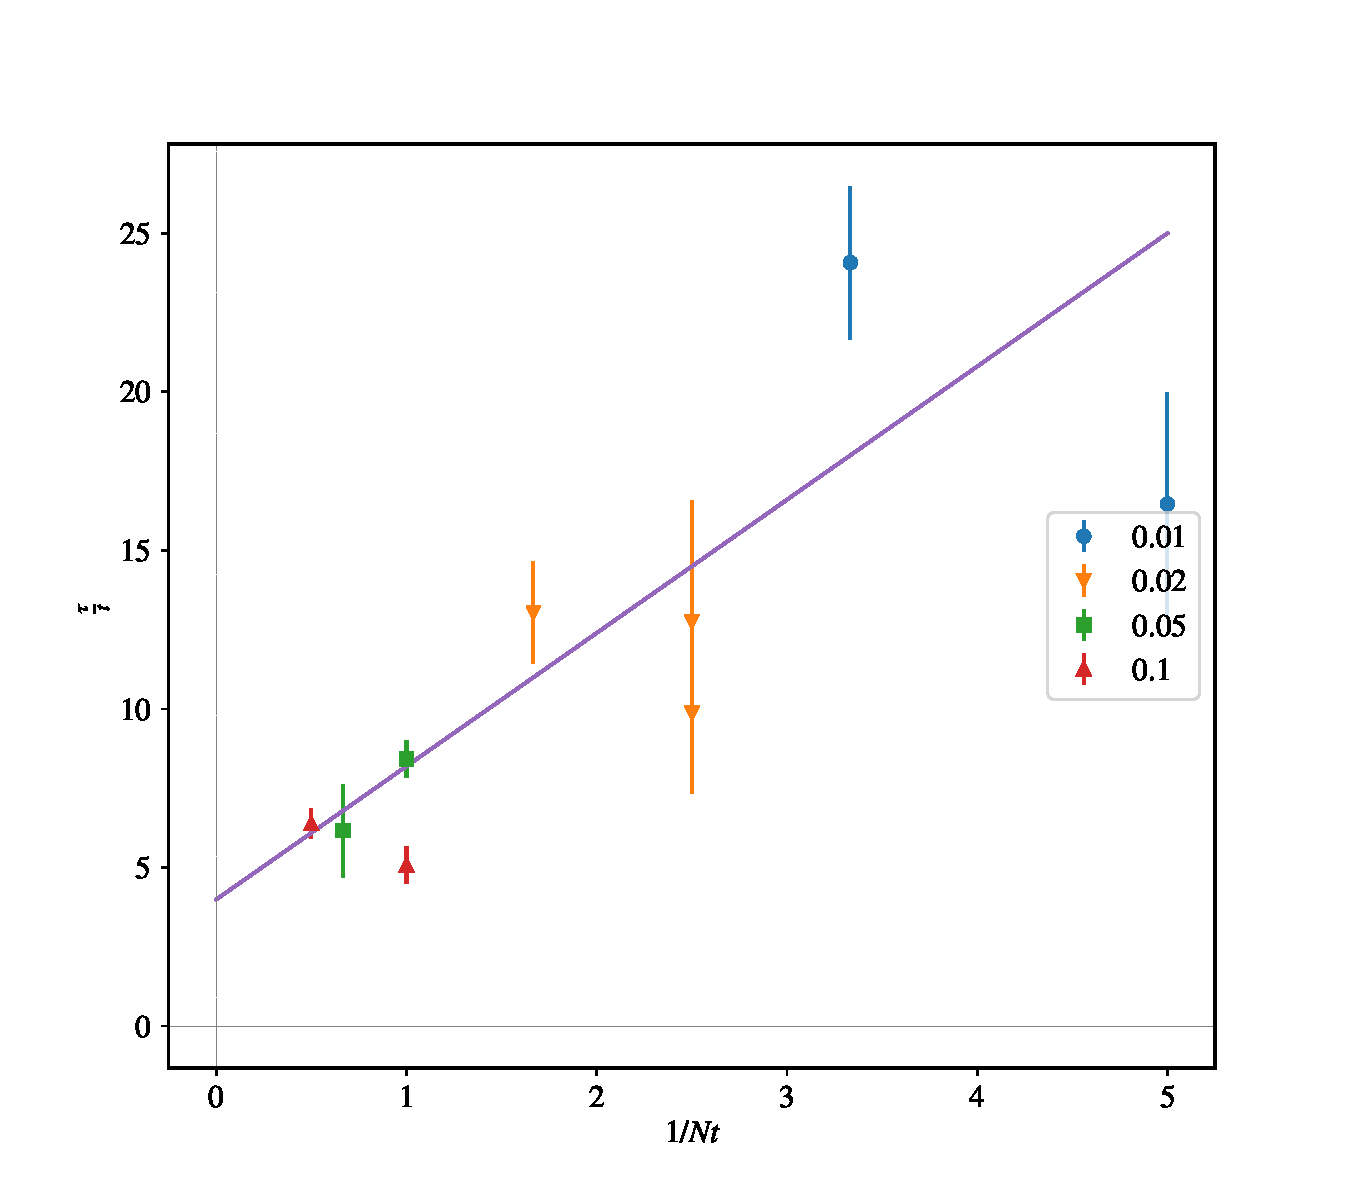
\includegraphics[width=.75\textwidth]{media/tau_TN}
  \caption{$\tau/t$ as a function of $\frac{1}{N t}$.\label{fig:tau_TN}}
\end{figure}


\section{Findings related to performance\label{sec:performance}}
During the development process, several benchmarks were made, and I discovered some small changes that had huge impact on performance.
Especially pices of code that are involved in the very core of the simulation loop, the flipping, are vital to streamline as they are executed several million, or even billion, times.

The most successful change I made with regards to performance, was also quite subtle.
At the core of the simulation, in the flipping attempt, the function \verb|step!| in my code, one has to calculate the interaction between neighbors.
In the old version of the neighbor interaction calculation I had the following snippet, generating a vector of neighbor spins.

%\begin{minipage}{\linewidth}
\begin{lstlisting}
  return [H[(y, x)] for (y,x) in [
      (y, ir[x]),  # Right
      (y, il[x]),  # Left
      (iu[y], x),  # Up
      (id[y], x),  # Down
  ]]
\end{lstlisting}
%\end{minipage}
Here, \verb|H| is the spin array and \verb|ir, il, iu, id| are the index vectors.
I changed this snippet to
\begin{lstlisting}
  return (y, ir[x])+  # Right
         (y, il[x])+  # Left
         (iu[y], x)+  # Up
         (id[y], x)   # Down
\end{lstlisting}
The difference between the two techniques is that the former makes a new a list, to which is applied the built in sum function while in the latter the sum is carried out directly, not having to allocate a list.
Also, the former is created with a loop.
However, even a list written out, not created using a list comprehension, is slower than the direct sum, with a factor of about 2.
This is in fact one of the points mentioned in Julia's page on performance tips, direct sum instead of summing over a list.
The change in performance was huge -- going from 34 seconds to 3.5 seconds in a benchmark with $N=30$ and hundred thousand sweeps.
That corresponds to cutting the computaton time from one hour to six minutes!

At one point, I changed the type of the index vectors from Int64 to UInt8, under the assumption that one would not simulate systems of $N=255$.
This would obviously save memory, but strangely it had a negative inpact on speed, with a factor of about 3.
I did not persue this in depth, so I do not now the reason for this.
My theory is that either there is something inherent with Julia or the computer that makes 64 bits faster, or that the compiler performs some hidden conversion of the UInt8.
The latter possibility could have been found by writing the code more strict in type, but I did not prioritize this.


One last point on performance is parallelization.
The simulation is very CPU-demanding, but not very memory expensive, and should be fit for running on multiple threads.
One simulation can not be multithreaded, as it has to be sequential, but running multiple simulations at once would be very benifical in leveraging the full potential of the CPU.
I did try to run two simulations in parallell, but they one was killed by the OS because of memory.
The memory issue did, however, not arise from the simulation itself, but from the bootstrapping.
The bootstrap-implementation is vectorized, all the random samples are genereted first, and then Julia's vectorized syntax is used.
Since we have to store all the random numbers, it is memory intentisive.
Two possible ways to solve this issue is to 1) store the results from the simulation to file and the do bootstrapping later or 2) see if one could ommit the problem by writing non-vectorizied code that requires less memory.
I did not persue this further, but it is definitely one of the first improvements it would be logical to attempt.


As a final note on parallelization, I will mention that I did very briefly attempt further optimization of the neighbor interaction calculation.
The neighbor interaction consists of accessing four spin values and summing them.
As mentioned, speeding up this operation is very impactful.
Utilizing the SIMD instructions for multiplying these four values would probably give a considerable speedup.
I did try this, but was not successful.

  |-> 30s -> 3.5s ( 1 hour -> 6 minutes of simulation )
- Only uses one core, and is fairly cheap on memory.
  Should be possible to run multiple at once.
  Problem that bootstrap uses much memory -> killed
  Solution: bootstrap later or non-vectorized


\begin{thebibliography}{9}
\bibitem{niels} M. E. J. Newman and G. T. Barkema, \emph{Monte Carlo Methods in Statistical Physics} chap. 3, Oxford University Press, Oxford, 1999.

\bibitem{onsager}  L. Onsager, \emph{Crystal statistics. I. A two-dimensional model with an order-disorder transition},  Phys. Rev. 65, 117 (1944).

\bibitem{mon_jasnow} ]  K.K. Mon and D. Jasnow, \emph{Direct calculation of interfacial tension for lattice models by the Monte Carlo method}, Phys. Rev. A 30, 670 (1984). 
\end{thebibliography}
\end{document}
